\documentclass[10pt,a4paper]{article}
\usepackage[margin=1.8cm]{geometry}
\usepackage[T1]{fontenc}
\usepackage{lmodern}
\usepackage{microtype}
\usepackage{graphicx}
\usepackage{booktabs}
\usepackage{amsmath}
\usepackage{xcolor}
\usepackage{tikz}
\usetikzlibrary{arrows.meta,positioning}
\usepackage[hidelinks]{hyperref}
\usepackage{enumitem}
\usepackage{caption}
\setlist{nosep,leftmargin=1.2em}
\setlength{\parskip}{3pt}
\setlength{\parindent}{0pt}
\graphicspath{{../figures/}{../screens/}}
\definecolor{ink}{HTML}{052F4A}
\definecolor{sky}{HTML}{0069A8}

\title{\textbf{Lodestar: an explainable cognitive growth agent}\\[2pt]
\large AI4Brain, CISTAC 1.0 --- technical report}
\author{AI4Brain team}
\date{October 2026}

\begin{document}
\maketitle
\vspace{-1.5em}

\begin{abstract}
\noindent Lodestar is an AI agent that assesses sixteen cognitive skills through short games, keeps a
dynamic, historised profile of each person (the \emph{Brain Twin}) in which every estimate carries an
80\% range, coaches in natural language with every number traced to a cited fact, and adapts
exercises, goals and plans as the profile changes. A LangGraph agent with 22 nodes decides what to do
next and records every decision with the options it weighed. A Kalman-Elo scoring engine turns
answers into estimates with honest uncertainty; four learned or statistical models forecast growth,
detect drifting engagement, find the fatigue point and pick the game that helps most. On 200
simulated people with known skills, the profile recovers the true skill with correlation 0.82 after
three sessions and 0.91 after ten, and its 80\% ranges contain the truth 79.9\% of the time. The
system runs without camera or microphone, without a cloud model, and degrades gracefully when its
models or memory are down. Lodestar is a practice coach; it never assesses medical or psychological
conditions.
\end{abstract}

\section{Objectives and scope}
The brief asks for an agent that \emph{assesses} the user across cognitive dimensions
non-clinically, \emph{understands} performance as an uncertainty-aware percentage profile,
\emph{coaches} with explainable, personalised feedback, and \emph{improves} through adaptive exercises
and measurable learning paths (Layers A--C), with an AI Collaboration Score, documented ethics, and
optional voice, emotion-aware and predictive features. Table~\ref{tab:map} maps each requirement to
the component that meets it. All three bonus features are implemented.

\begin{table}[h]
\centering\small
\begin{tabular}{@{}p{4.2cm}p{12.2cm}@{}}
\toprule
Requirement & Lodestar \\
\midrule
A: tasks per dimension; score, RT, errors, behaviour & 43 browser games over 16 skills; every trial stores correctness, response time, hint level, practice flag and optional confidence \\
A: each dimension documented & Generated skill pages: definition, tasks, scoring, uncertainty, biases and evidence level \\
A: non-biometric mode mandatory & The default; camera and voice tone are off, per-switch consented, and never write to the profile \\
Brain Twin: history; projections with uncertainty & Append-only event log, daily history, growth forecast as an 80\% range \\
B: explainable coaching, no clinical terms & Facts packet $\to$ draft $\to$ verify $\to$ repair; citations on every number; banned-word check in lint and at runtime \\
C: adaptation, plans, radar, curves, heatmaps, goals & Difficulty targeting, bandit, goals, personal experiments; all four chart types with ranges \\
AI Collaboration Score (0--100, formula) & Five components measured in play; Bayesian shares; documented weights and sensitivity \\
Ethics \& data & Layered consent, export, deletion with receipt, retention job, encrypted user keys \\
Bonus & Voice in/out with wake word; on-device strain cues; predictive growth \\
\bottomrule
\end{tabular}
\caption{Brief requirements and where they are met.}\label{tab:map}
\end{table}

\section{Architecture}
\begin{figure}[h]
\centering
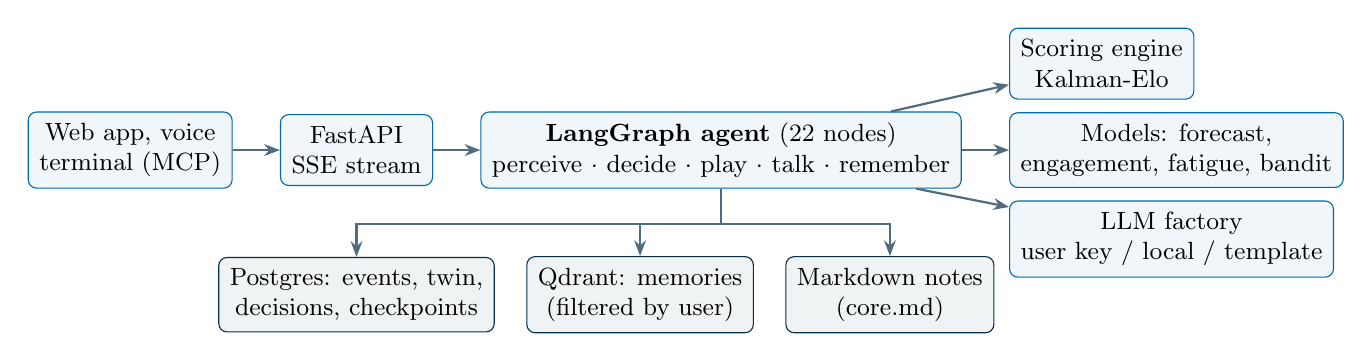
\begin{tikzpicture}[
  box/.style={draw=sky,rounded corners=3pt,fill=sky!6,align=center,font=\small,minimum height=0.9cm,inner sep=4pt},
  st/.style={draw=ink,rounded corners=3pt,fill=ink!6,align=center,font=\small,minimum height=0.9cm,inner sep=4pt},
  ar/.style={-{Stealth[length=2mm]},thick,color=ink!70}]
\node[box] (ui) {Web app, voice\\terminal (MCP)};
\node[box,right=0.6cm of ui] (api) {FastAPI\\SSE stream};
\node[box,right=0.6cm of api,minimum width=4.2cm] (g) {\textbf{LangGraph agent} (22 nodes)\\perceive $\cdot$ decide $\cdot$ play $\cdot$ talk $\cdot$ remember};
\node[box,above right=0.15cm and 0.6cm of g] (sc) {Scoring engine\\Kalman-Elo};
\node[box,right=0.6cm of g] (ml) {Models: forecast,\\engagement, fatigue, bandit};
\node[box,below right=0.15cm and 0.6cm of g] (llm) {LLM factory\\user key / local / template};
\node[st,below=0.9cm of api] (pg) {Postgres: events, twin,\\decisions, checkpoints};
\node[st,right=0.4cm of pg] (q) {Qdrant: memories\\(filtered by user)};
\node[st,right=0.4cm of q] (md) {Markdown notes\\(core.md)};
\draw[ar] (ui)--(api); \draw[ar] (api)--(g); \draw[ar] (g)--(sc); \draw[ar] (g)--(ml); \draw[ar] (g)--(llm);
\draw[ar] (g.south)--++(0,-0.45)-|(pg.north); \draw[ar] (g.south)--++(0,-0.45)-|(q.north); \draw[ar] (g.south)--++(0,-0.45)-|(md.north);
\end{tikzpicture}
\caption{System overview. Postgres is the system of record; Qdrant holds searchable memories; Markdown holds the notes Lodestar writes.}
\label{fig:arch}
\end{figure}

\textbf{Why this architecture.} A graph agent (LangGraph~1.2) rather than a free-form tool loop makes
every step inspectable and resumable: state is checkpointed in Postgres, so a browser crash in the
middle of a game resumes on the same trial. Deterministic code decides \emph{what} to do (which skill,
which game, which difficulty) and records the decision with its candidates and the parts of each score;
the language model only decides \emph{how to say it}, from a facts packet. This split keeps decisions
explainable and testable, keeps every number traceable, and lets the app run with a small local model
or none at all. Users bring their own key for eight hosted providers, or use a local Ollama model; keys
are encrypted at rest and decrypted only inside the LLM factory. All storage is Postgres (structured
data, append-only events), Qdrant (memory search, always filtered by user) and readable Markdown notes.

\section{Assessment and the Brain Twin}
\textbf{Skills and tasks.} Sixteen skills are grouped into attention, self-control, memory, speed,
reasoning and language, each tagged \emph{established}, \emph{moderate} or \emph{experimental} by the
strength of its evidence. Classic paradigms (flanker, Stroop, n-back, Corsi, go/no-go, task
switching, digit span, mental rotation, Tower of London, matrices) are rebuilt from their published
descriptions, alongside original games and a Detective story whose chapters are games. A registry in
YAML describes every game (skills and loadings, scoring, difficulty knobs, practice trials) and drives
the UI, the scorer and the agent alike. A five-minute warm-up battery measures the core skills first.

\textbf{Scoring.} Each skill $d$ has a belief $\theta_d\sim\mathcal N(\mu,\sigma^2)$ on a logit scale,
each level a difficulty $b$. For an answer with outcome $S$ (timed tasks use a high-speed high-stakes
rule: right \emph{and} within the reference pace),
\begin{align*}
p &= \operatorname{logistic}\!\Big(\tfrac{\mu-b}{\sqrt{1+\pi\sigma^2/8}}\Big), &
w &= \text{loading}\times\text{reliability}\times\text{trust}, \\
\sigma'^2 &= \big(1/\sigma^2 + w\,p(1-p)\big)^{-1}, &
\mu' &= \mu + \sigma'^2\, w\,(S-p).
\end{align*}
Uncertainty grows with time away ($\sigma^2\leftarrow\min(\sigma_0^2,\sigma^2+q\,\Delta t)$) and with
within-session process noise; a practice prior fitted to 1.08 million Lumosity learning curves moves
$\mu$ by the expected gain per round. Cold-start priors come from skill correlations computed on
180{,}000 NCPT test runs. Estimates are shown as percentiles with 80\% ranges
($\mu\pm1.28\sigma$), labelled ``simulated norms'' until a linking study maps our scale onto
published norms. Rounds that look like bad data (too fast, flat responding, outliers) are flagged and
down-weighted rather than trusted.

\textbf{History.} A scored round is one transaction: events, trials, round, profile and daily
history, under a per-user advisory lock. Events are never updated, so the whole profile can be rebuilt
from the log. The Brain Twin shows each skill as a card (estimate, range bar, a shadow that widens
with uncertainty), wired to skills of the same family and to the skills it correlates with most.

\section{The AI coach and explainability}
Each reply is built in three steps. The agent assembles a \emph{facts packet} (numbered facts,
decisions, knowledge tips and memories, each with an id); the LLM drafts in the chosen voice (Willow,
Spark, Sage or Buddy); a verifier rejects any number not found in a cited fact, any banned clinical
word and any unsupported claim, asks for a repair, and falls back to a template if the repair fails.
In the UI every cited number shows its chip (\texttt{[F2]}), and ``Why?'' opens the decision behind a
game: the candidate skills, the score of each, and its parts (uncertainty, staleness, goal weight,
bandit gain, fatigue, repetition). The Agent page shows the five stages lighting up live and every
decision with the options it weighed; the full trace is stored per session. With the local
\texttt{qwen3.5:4b} model, 1 of 4 first drafts passed verification, 3 after repair and 1 by
template: 4 of 4 final replies were faithful, which is the point of the loop.

\begin{figure}[h]
\centering
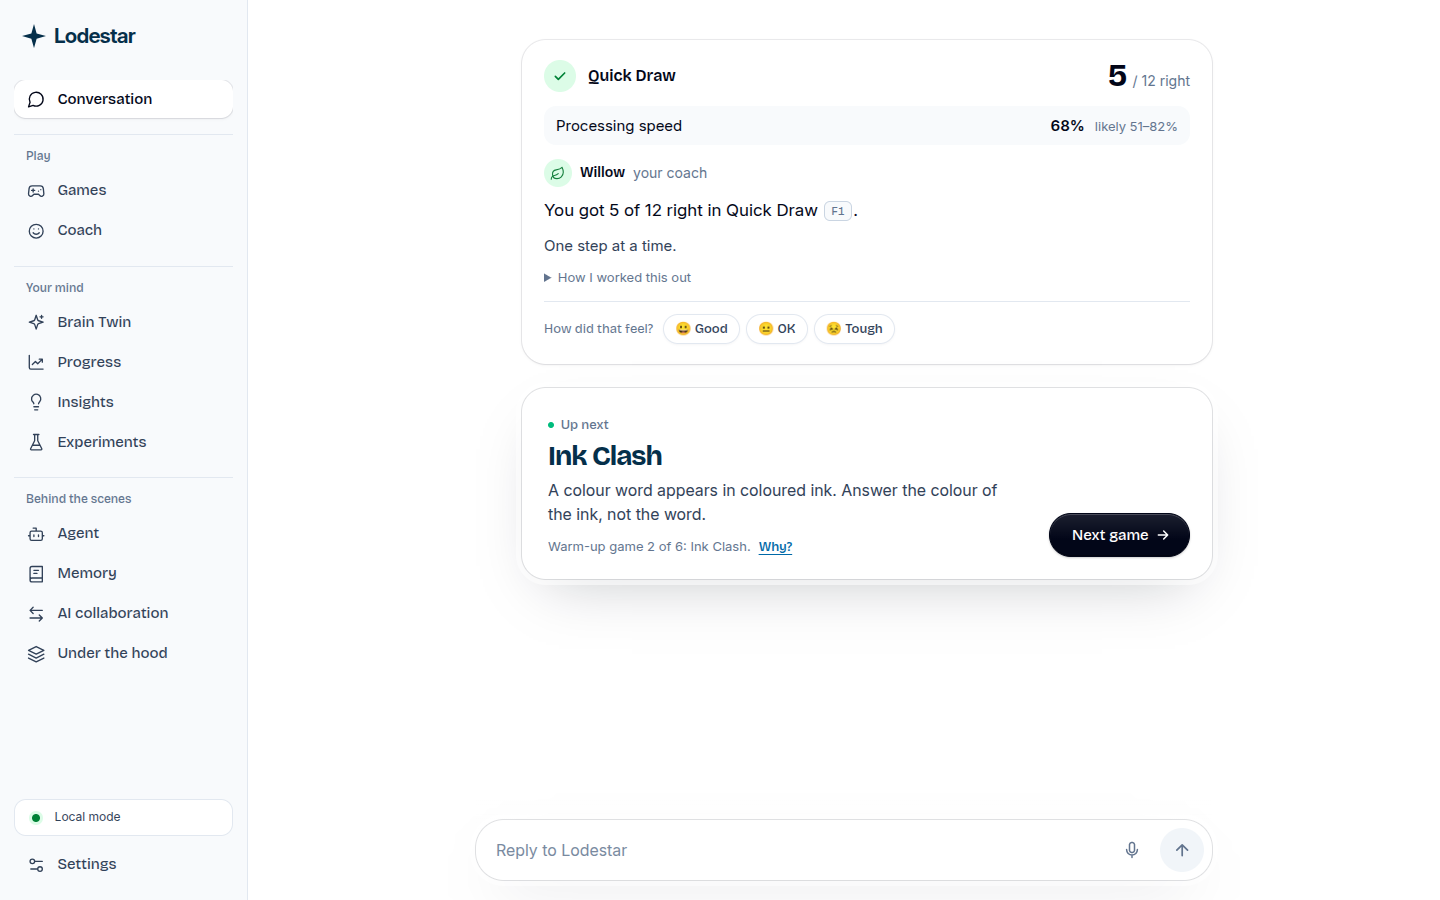
\includegraphics[width=0.49\linewidth]{result.png}\hfill
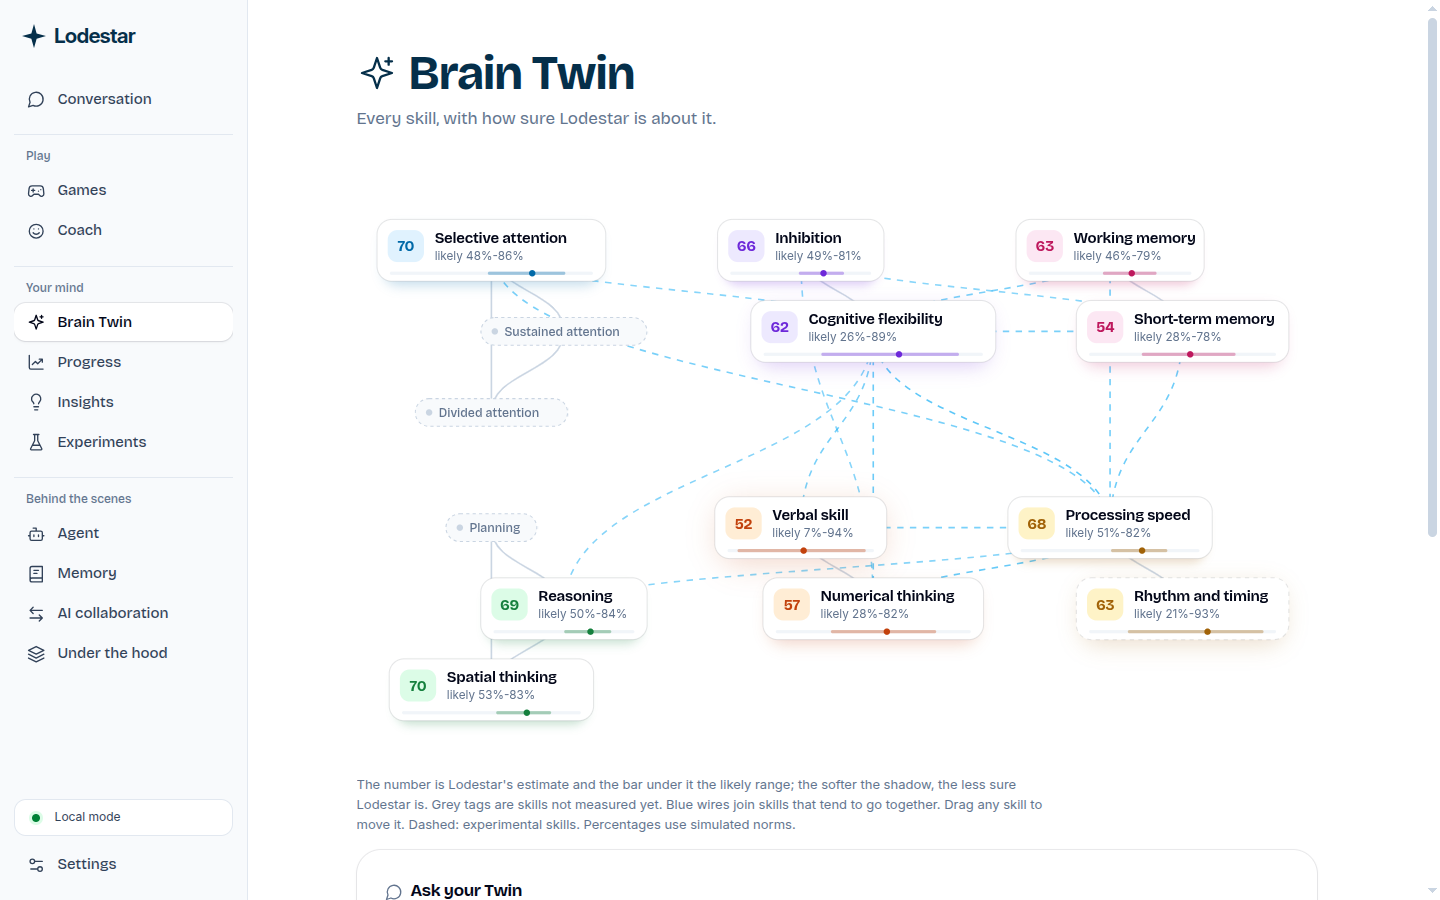
\includegraphics[width=0.49\linewidth]{twin.png}
\caption{Left: after a game, the score, the skill it moved with its range, and the coach with a cited fact. Right: the Brain Twin, each skill a card with its estimate and range.}
\end{figure}

\section{Adaptive learning and the dashboard}
\textbf{Difficulty} targets the success rate the user chose (Chill, Balanced or Push):
$b_{\text{next}}=\mu-\operatorname{logit}(p^*)$, with an in-game staircase. On the simulator,
Balanced mode achieved 77.7\% success against an 80\% target. \textbf{What to play} is chosen by a
weighted score over skills (uncertainty, staleness, goals, experiments, fatigue, repetition) plus a
Thompson-sampling bandit that learns which game moves each skill most for this person (+0.12 to
+0.24 true-skill gain over random games, 95\% interval). \textbf{Plans evolve}: goals are stated as
``know this skill to within $\pm N$ points by a date'', with rounds left estimated from the update
rule; personal experiments compare morning and evening sessions and report a verdict only when
$P(\text{one is better})\ge0.8$. The dashboard has the radar, progress curves with forecast bands and
life-context strips, heatmaps by week and time of day, and goal cards; every estimate shows its range.

\begin{figure}[h]
\centering
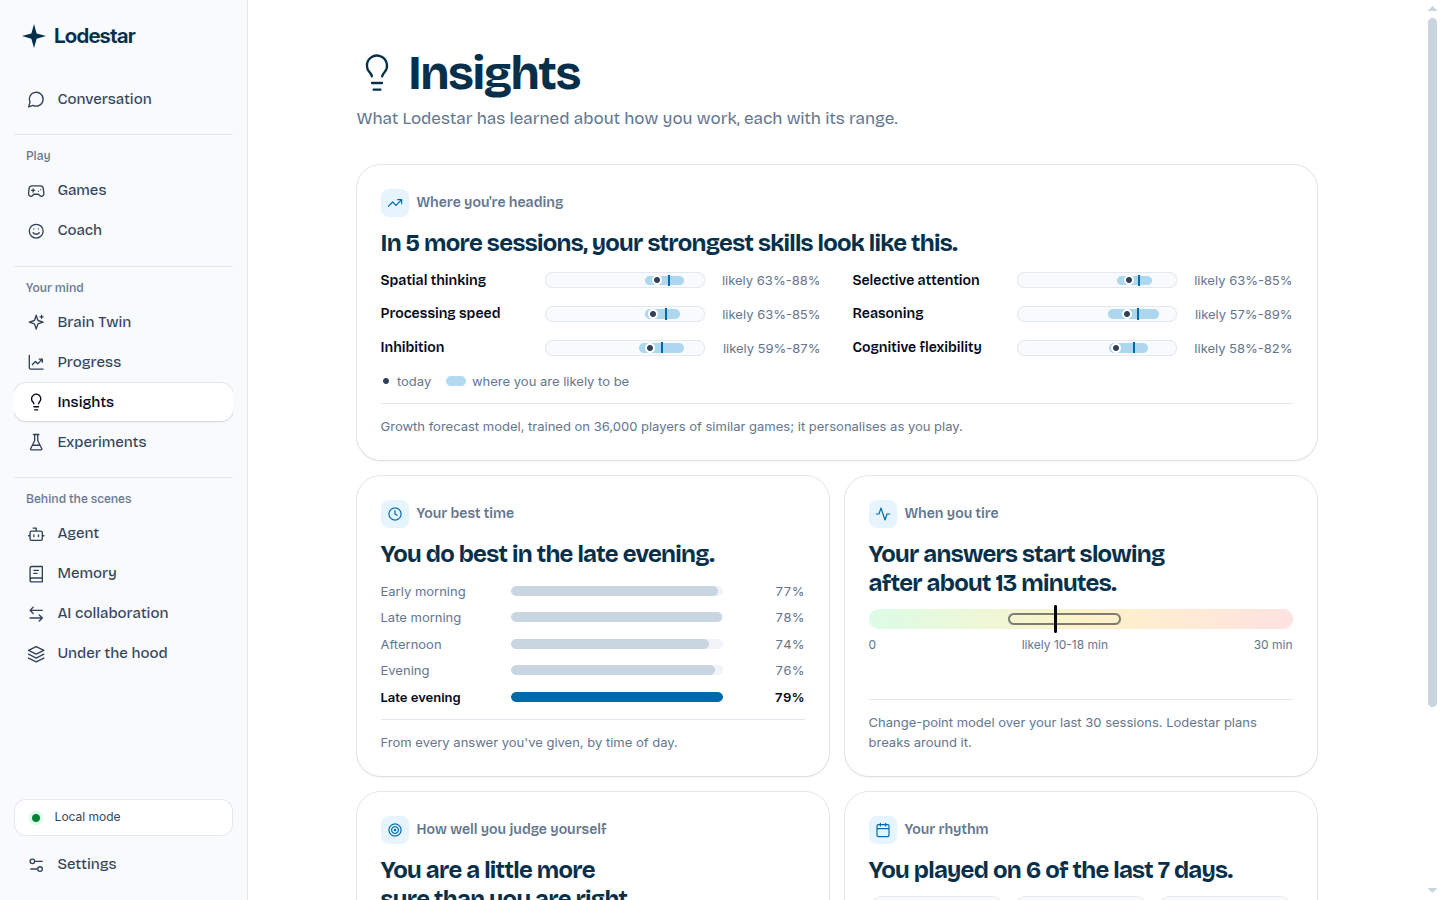
\includegraphics[width=0.49\linewidth]{insights.png}\hfill
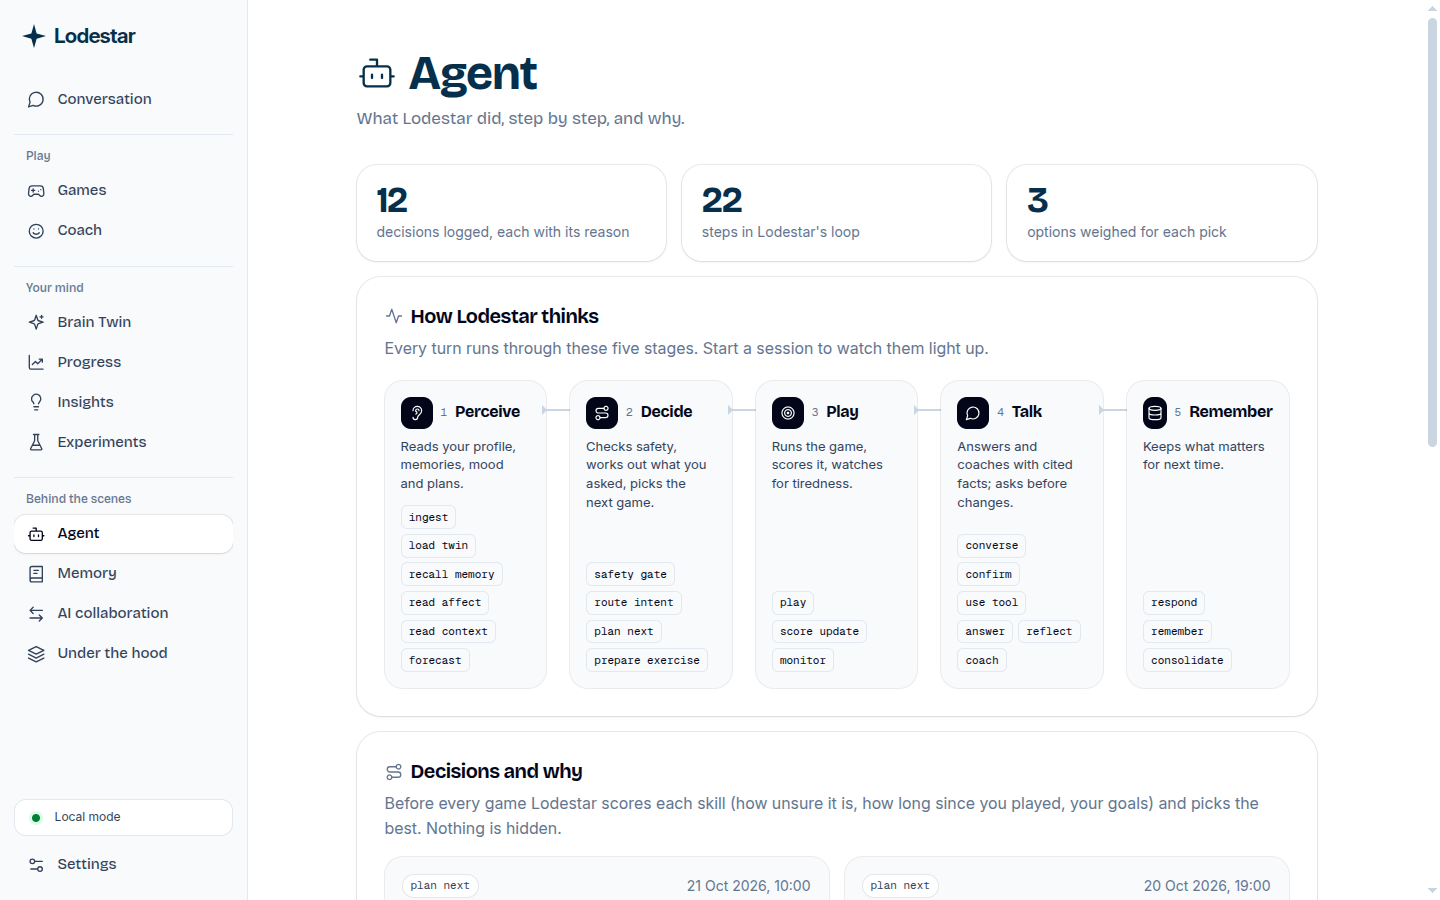
\includegraphics[width=0.49\linewidth]{agent.png}
\caption{Left: Insights, each reading with its range and the model behind it. Right: the Agent page, the five stages and the decisions with their reasons.}
\end{figure}

\section{AI Collaboration Score}
Each of five components is measured inside games: critical verification (finding planted mistakes
in the AI's worked solutions, with consent), autonomy (solving before asking for a hint), iteration
(a better retry after a failure), clarification (asking before acting on an ambiguous instruction)
and responsible use (taking a suggested break). With a Beta(2,2) prior per component,
\[
s_k=\frac{\text{successes}_k+2}{\text{opportunities}_k+4},\qquad
\text{ACS}=100\sum_k w_k s_k,
\]
and an 80\% range from 1{,}000 Monte Carlo draws. Weights are V\,0.30, A\,0.20, I\,0.20, C\,0.15,
R\,0.15: verification is raised from the brief's 0.25 because over-reliance is the main failure mode
of AI assistance, clarification lowered because its opportunities are rarest. Ranks are stable under
$\pm5$-point weight changes (worst Spearman 0.997 on 200 simulated people).

\section{Predictive models}
\begin{itemize}
\item \textbf{Growth forecast.} LightGBM quantile models (10/50/90) with split-conformal calibration,
trained on 36{,}297 users of Steyvers \& Schafer's open Lumosity data and evaluated on held-out
\emph{users}: observed 80\% interval coverage 79.6--80.0\% for horizons of 1 to 20 sessions. In the app a
person's own history outweighs the population forecast as data accumulate.
\item \textbf{Engagement risk.} Logistic regression on eight behaviour features, trained on OULAD
(25{,}273 students); held-out AUC 0.857 (LightGBM 0.863, days-since-last rule 0.828) with an inductive
Venn--Abers range (ECE 0.006). It only ever triggers a shorter, easier session; the score is never shown.
\item \textbf{Fatigue point.} A change-point detector on standardised log response times per session,
combined with a Kaplan--Meier curve across sessions, gives the minute at which answers start slowing
(median with its middle half). Sessions where the person slowed but became more accurate are excluded.
\item \textbf{Best next game.} The Thompson-sampling bandit above, updated from every round.
\end{itemize}

\begin{figure}[h]
\centering
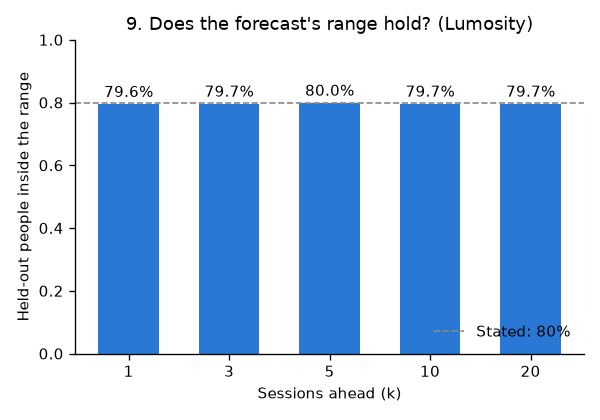
\includegraphics[width=0.48\linewidth]{eval_09_forecast.png}\hfill
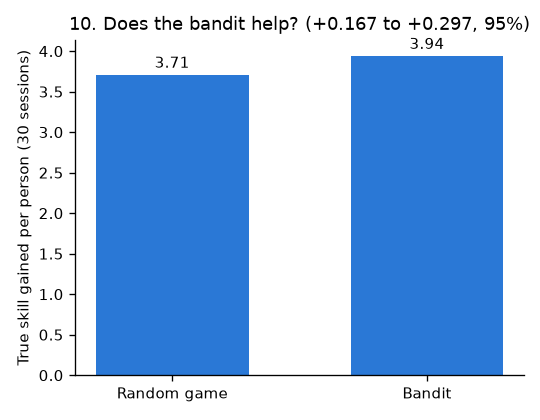
\includegraphics[width=0.48\linewidth]{eval_10_bandit.png}
\caption{Left: the growth forecast's 80\% ranges hold on held-out real players at every horizon. Right: true-skill gain with the bandit versus random games.}
\end{figure}

\section{Evaluation}
A simulator draws 200 people with known true skills (correlated as in NCPT), plays ten sessions each
through the scoring and selection code, and checks the profile against the truth.
Table~\ref{tab:eval} summarises the eleven experiments; figures are in the repository.

\begin{table}[h]
\centering\small
\begin{tabular}{@{}lll@{}}
\toprule
Question & Result & Target \\
\midrule
Recovery of true skill (correlation), after 1 / 3 / 10 sessions & 0.773 / \textbf{0.820} / 0.905 & $>0.8$ at 3 \\
80\% ranges containing the true skill & \textbf{79.9\%} & 75--85\% \\
Achieved success in Balanced mode & 77.7\% & $80\pm5\%$ \\
Worst core-skill $\sigma$ after the warm-up & 0.65 & $<0.8$ \\
Bad-data detection, precision / recall & 1.00 / 1.00 & $>0.9$ / $>0.8$ \\
RMSE after 10 sessions: usual / long gaps / 50--150 ms lag & 0.449 / 0.479 / 0.535 & reported \\
ACS rank stability under weight shifts (Spearman) & 0.997 & $>0.9$ \\
Coach faithfulness, final replies (local 4B model) & 4/4 & 100\% \\
Forecast coverage on held-out real players & 79.7\% & 80\% \\
Bandit gain over random games (95\% interval) & +0.12 to +0.24 & reported \\
Sessions completed with all models down / Qdrant down / both & 18/18 each & 100\% \\
\bottomrule
\end{tabular}
\caption{Evaluation (\texttt{make eval}, seed 2026).}\label{tab:eval}
\end{table}

\begin{figure}[h]
\centering
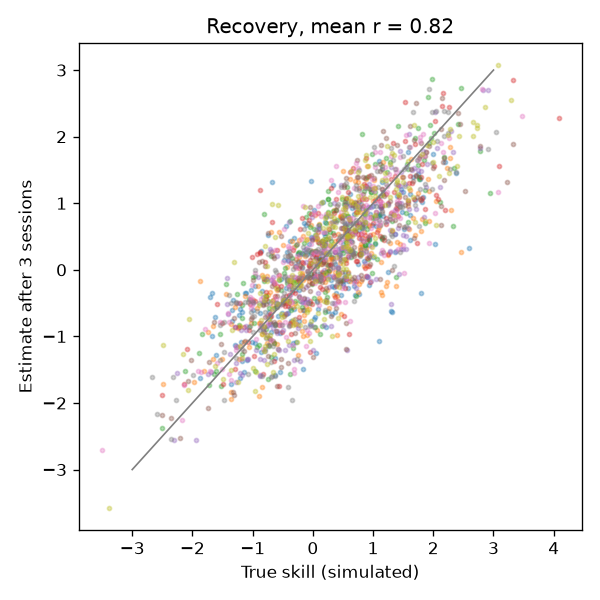
\includegraphics[width=0.48\linewidth]{sim_recovery.png}\hfill
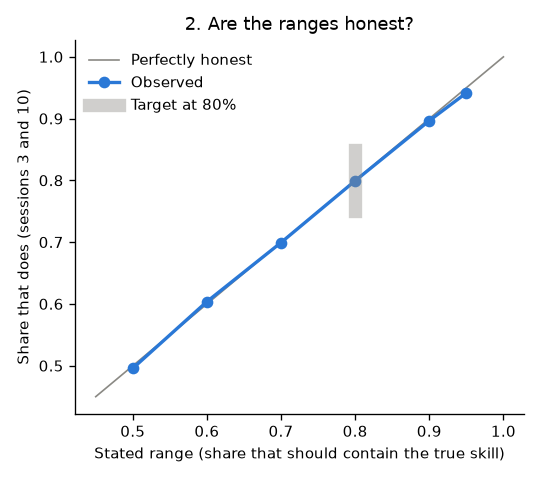
\includegraphics[width=0.48\linewidth]{eval_02_ranges.png}
\caption{Left: recovery of true skill by session. Right: coverage of the 80\% ranges.}
\end{figure}

\textbf{Generalisation and robustness.} The models that touch real people were evaluated on held-out
real users from public data (Lumosity, OULAD), not on the people they were trained on. Experiments 1--5
also run through the full agent graph (\texttt{make sim-graph}), and the system was tested with
sessions weeks apart, device lag, every model failing and the memory store unreachable. The software
is covered by 265 backend tests, 84 frontend unit tests and 14 end-to-end suites in a real browser,
run in CI.

\begin{figure}[h]
\centering
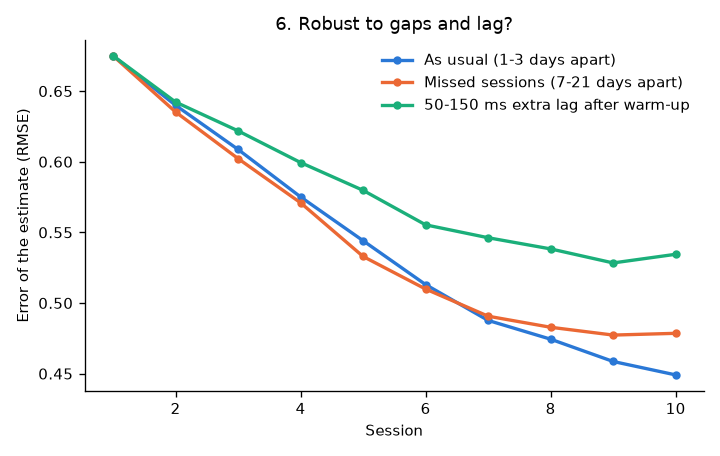
\includegraphics[width=0.48\linewidth]{eval_06_gaps_lag.png}\hfill
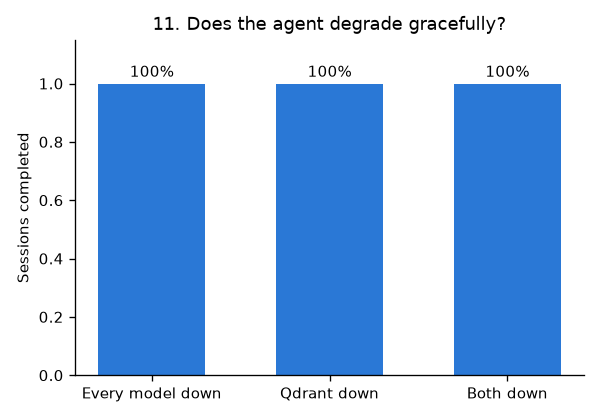
\includegraphics[width=0.48\linewidth]{eval_11_degradation.png}
\caption{Robustness. Left: error after long gaps and with device lag. Right: sessions completed through the real agent with models, memory, or both unavailable.}
\end{figure}

\section{Ethics, safety and data}
Seven consent switches (core data, cloud AI, microphone, camera, voice tone, planted-mistake games,
research export) are logged as events with the notice version; nothing is stored before the
first-visit screens finish, and the app is for adults (18+). Camera and voice-tone cues are computed
on the device, sent as one coarse number each, used only to suggest a break, and have no code path to
the profile; no decision rests on face or voice alone. Users can read and forget any memory line,
export everything, or delete everything and receive a receipt with the counts removed; a daily
retention job removes old traces, checkpoints and events. Cloud AI receives only de-identified
summaries. A banned-word list (diagnostic and clinical terms) is enforced in CI and in every reply,
and a red-team suite checks requests for diagnoses. User API keys never appear in state, logs or
exports.

\section{Limitations and next steps}
Validity rests on established paradigms and on the simulator, not yet on a study with real Lodestar
users; percentiles use simulated norms until a linking study puts our scale against NCPT; the
engagement model transfers from online courses to games; experimental skills (rhythm, creativity,
accuracy awareness) are labelled as such. Next: a consented pilot with 5--10 people (usability, whether
``why'' cards are understood, labels for the frustration cues), a linking study for norms, and more
languages.

\section*{References}
\small
Klinkenberg, Straatemeier \& van der Maas (2011), Computer adaptive practice of Maths ability using a
new item response model for on the fly ability and difficulty estimation. \emph{Computers \& Education}.
Jaffe et al. (2022), NCPT, \emph{Scientific Data}. Steyvers \& Schafer (2020), \emph{Nature Human
Behaviour}. Kuzilek, Hlosta \& Zdrahal (2017), OULAD, \emph{Scientific Data}. Bu\c{c}inca, Malaya \&
Gajos (2021), To trust or to think, \emph{CSCW}. Vovk et al. (2015), Venn--Abers predictors.
\end{document}
